% $Id: magarch-april2000.tex 204 2009-04-20 01:59:36Z jsibert $
%
% Author: David Fournier
% Copyright (c) 2008 Regents of the University of California
%

The Vector Autoregressive Moving Average Garch process combines
the Vector Autoregressive Moving Average (\textsc{varma})
processes with the Vector Garch (generalized 
autoregressive conditional heteroscedastic) processes.


\section{Formulation of the \textsc{varma garch} process}

The \textsc{varma garch} process of type $(p,q,r,s)$ is given by a 
series $Y_t$ for $t=-p+1,\ldots,n$, where for each value of $t$,
$Y_t$ is an $m$-dimensional vector.
For $t>0$, the $Y_t$ are assumed to satisfy a relationship of the form
\begin{equation}
  Y_t=\mu +\sum_{l=1}^p A_l (Y_{t-l}-\mu)
    +\sum_{l=0}^q B_l \epsilon_{t-l}            
  \label{eq1}
\end{equation}
where the $\mu$ is an $m$-dimensional vector, 
$A_l$ and $B_l$ are $m\times m$ matrices, $B_0$ is the identity
matrix,  and the
$\epsilon_t$ are multivariate (normal) random vectors,
with means~$0$.  Covariance matrices $\Sigma_t$ and
 $\hbox{\rm E}(\epsilon_t\epsilon_{t^\prime})=0$ if $t\ne t^\prime$.
Let
\begin{equation}
  r_t=Y_t-\mu -\sum_{l=1}^p A_l (Y_{t-l}-\mu)
  \label{eqc1}
\end{equation}
be the vector of model residuals or ``shocks.''\footnote{For the moving
average model ($q>0$), one might argue that since the previous values
of $r_t$ have been observed, the shock part of $r_t$, say,
$d_t$, is given by $d_t=r_t-\sum_{l=1}^q B_l r_{t-l}$,
but this has not been done at present.}
These residuals are
assumed to contribute to the covariance matrix in the next time period.
The $\Sigma_t$ evolve according to one of several relationships.

\subsubsection{The \textsc{dvec} relationship}
\begin{equation}
  \Sigma_t=\Omega+
        \sum_{l=1}^r F_l\bigotimes r_{t-l}r_{t-l}^\prime  
         +\sum_{l=1}^sG_l\bigotimes \Sigma_{t-l}
  \label{eqc}
\end{equation}
In equation~(\ref{eqc}), the matrices 
$F_l$ and $G_l$ are symmetric and the operator
`$\bigotimes$' denotes the element-wise product of matrices.
This parameterization does not restrict the resulting matrix to
be positive definite, so some care is necessary to ensure the
stability of the resulting~model.

\subsubsection{The \textsc{bekk} relationship}
\begin{equation}
\Sigma_t=\Omega+
       \sum_{l=1}^r F_l\, r_{t-l}\, r_{t-l}^\prime\, F_l^\prime 
        + \sum_{l=1}^s\, G_l\, \Sigma_{t-l}\, G_l^\prime
  \label{eq2}
\end{equation}

\subsubsection{\textsc{dveci} and \textsc{bekkai} parameterizations}
The basic \textsc{dvec} and \textsc{bekk} parameterizations can be extended by  modifying
components of the $r_t$ to reflect the asymmetric response
to positive and negative values.
\begin{align}
    \nonumber \eta_{ij} =&\epsilon_{ij}/\alpha_j &\textrm{if } \epsilon_{ij} \ge 0\\
    \eta_{ij} =&\epsilon_{ij}\alpha_j                    &\textrm{if }  \epsilon_{ij} < 0
\end{align}
This modified form will be referred to as the \textsc{dveci} and \textsc{bekkai} parameterizations.
\begin{equation}
\Sigma_t=\Omega+
        \sum_{l=1}^r F_t\bigotimes \eta_{t-l}\, \eta_{t-l}^\prime  
         +\sum_{l=1}^sG_l\bigotimes \Sigma_{t-l}
  \label{eqd}
\end{equation}
\begin{equation}
  \Sigma_t=\Omega+
       \sum_{l=1}^r F_l\, \eta_{t-l}\, \eta_{t-l}^\prime\, F_l^\prime 
        + \sum_{l=1}^sG_l\, \Sigma_{t-l}\, G_l^\prime
   \label{eqe}
\end{equation}


\section{Setting a value for $\Sigma_1$}

The value for the parameters in $\Sigma_1$ are often poorly determined 
and simply letting them be free parameters can lead to 
instability and initial
transient effects in the model. To stabilize the parameterization, we have 
calculated $\Sigma_1$ through $\Sigma_{\max\{r,s\}}$ from the condition
\begin{equation}
  \widehat\Omega=\Sigma+\sum_{l=1}^q B_l\Sigma B_l^\prime 
\end{equation}
where 
\begin{equation}
  \widehat\Omega=\frac{1}{n}\sum_{t=1}^n\hat\epsilon_t\, \hat\epsilon_t^\prime 
\end{equation} 
denotes the empirical covariance matrix formed from the
models residuals 
\begin{equation}
  \hat\epsilon_t=Y_t-\mu-\sum_{l=1}^p A_l (Y_{t-l}-\mu).
\end{equation}


\section{Ensuring that the $\Sigma_t$ are positive definite}

The \textsc{dvec} parameterization can produce matrices that are not
positive definite, and the \textsc{bekk} parameterization can produce matrices
that are almost not positive definite (much as a positive number can
get arbitrarily close to zero). At worst, this will lead to a failure
in the model to converge and at best, it makes the estimation somewhat
unstable. To improve model performance, the \textsc{bekk} and \textsc{dvec}
operations are followed by a modification of the resulting $\Sigma_t$ that
 makes them more positive definite. The first problem is to get a notion of what is meant by ``small'' for a particular problem. 
This is accomplished by first scaling the 
$\Sigma_t$ to produce a matrix $\Lambda_t$ where
\begin{equation}
  \Lambda_{ij}=\frac{\Sigma_{t_{ij}}}{\sqrt{\Sigma_{t_{ij}}\Sigma_{t_{ij}}}}
\end{equation}
The terms $\Lambda_{ii}$ are then bounded above {$1.0\e{-3}$,  i.e., they are replaced in a differentiable fashion with numbers that are $\ge 1.0\e{-3}$ using
the \texttt{posfun} function.
In addition, the correlation matrix 
$\Lambda_{ij}/\sqrt{\Lambda_{t_{ij}}\Lambda_{t_{ij}}}$ is
decomposed via a Choleski decomposition, the divisors of
 which is forced to be $> 0.3$ in a differentiable fashion using the
\texttt{posfun} function.
\X{\fontindexentry{tt}{posfun} function}
The
above operations leave a matrix that is sufficiently positive definite
and close enough to $\Sigma_1$ unchanged.


\section{Missing data}

Missing data points are included into the model as parameters to
be estimated. If there are a substantial number of missing data
points, this will induce bias into the estimates.


\section{The likelihood function}

The model was fit by maximum-likelihood or, more correctly, by
finding the mode of the Bayesian posterior distribution.
A robust likelihood function that is a mixture of a normal
distribution and a Cauchy distribution is employed.  The amount of robustness
can be changed by the user.


\section{Model selection}

Model selection consists of fitting the model to the data for various values
of the parameters $(p,q,r,s)$ and trying to determine the simplest model
that adequately fits the data, if any. 

The two criteria which are used for this are the likelihood ratio test
and investigation of the residuals in the form of the Box-Ljung statistic.
The likelihood-ratio test is used for general model selection, while
the Box-Ljung statistic is used to investigate whether or not the model
can adequately fit the changes in the covariance matrices $\Sigma_t$
that occur over time.


\section{The Box-Ljung statistic}

The following Box-Ljung
Statistic was employed 
to test the ability of the model to model the time varying covariance
structure of the time series. This statistic is calculated from the
estimated standardized residuals $z_t$, for $t=1,\ldots n$,
where for each $t$, $z_t$ is an $m$-dimensional vector.
The $z_i$ are obtained in the calculations necessary to calculate the
log-likelihood~\mbox{function}.
\begin{align}
  \hat\mu_j&=\frac{1}{ n}\sum_{i=1}^n z_{ij}\\
  z_{ij}^{\prime}&=z_{ij}-\hat\mu_j\\
  \hat\sigma_{jk}&=\frac{1}{ n}\sum_{i=1}^n z_{ij}^\prime z_{ik}^\prime\\
  \gamma_{ijk}&=
       \frac{
            \frac{1}{ n-l}\sum_{i=1}^{n-l}
         (z_{ij}^\prime z_{ik}^\prime-\hat\sigma_{jk})
         (z_{i,j+l}^\prime z_{i,k+l}^\prime-\hat\sigma_{jk})
            }{                              
            \frac{1}{ n}\sum_{i=1}^n
         (z_{ij}^\prime z_{ik}^\prime-\hat\sigma_{jk})^2
       }
\end{align}

Under the null hypothesis that the model is adequate, and if the
$z_i$ are normally distributed, then the sum
$$LB(K)_{ij}=n\sum_{k=1}^k w_k \gamma_{ijk}^2$$
is asymptotically distributed as a $\chi^2$ random variables 
with~$K$ degrees of freedom. Here, $w_k=(n+2)/(n-k)$.


\section{Analysis of simulated data}

One method to get an idea how well a statistical model works is to
use it with simulated data where the true values of the parameters being estimated
are known.
A simple simulator that can generate data sets is included with the
\texttt{mgarch} package. The simulator generated a 4-dimensional set of
1,000 observations. A type~$1,1,1,1$ process was simulated and
analyzed.

The following plots show the actual and predicted values for the
diagonal variance and correlation terms for the analysis with
a type $1,1,1,1$~model.

\includegraphics[height=2.5in, width=\textwidth]{covarplot11.png}



\includegraphics[height=2.5in, width=\textwidth]{covarplot11.png}

\includegraphics[height=2.5in, width=\textwidth]{covarplot22.png}

\includegraphics[height=2.5in, width=\textwidth]{covarplot33.png}


\includegraphics[height=2.5in, width=\textwidth]{covarplot44.png}

\includegraphics[height=2.5in, width=\textwidth]{corrplot21.png}

\includegraphics[height=2.5in, width=\textwidth]{corrplot31.png}

\includegraphics[height=2.5in, width=\textwidth]{corrplot32.png}

\includegraphics[height=2.5in, width=\textwidth]{corrplot41.png}

\includegraphics[height=2.5in, width=\textwidth]{corrplot42.png}


\includegraphics[height=2.5in, width=\textwidth]{corrplot43.png}



\section{Analysis of real data}

The data consist of daily observations of the German Mark/US Dollar and Japanese Yen/US dollar exchange rates, as well as the SP-500 and Tokyo 
 (\textsc{tokyose}) stock exchange indices. For this data set, $m=4$, and there
were $1301$ time periods with $211$ missing values.  

\subsection{Model Parameters log-likelihood directory $p,q,r,s$.}
\begin{lstlisting}
VARMA
0,0,0,0   221         -1382.56      000
1,0,0,0   241         -1322.47      100
1,1,0,0   253         -1308.57      110

VARMA with DVEC
0,0,1,1   241         -1050.87 
1,1,2,1   283         -928.518 
1,2,1,1   289         -924.755  

VARMA with DVECI
1,1,2,1a  287         -887.764 
1,2,1,1a  293         -888.531 
\end{lstlisting}

\bigskip
\subsection{Ljung-Box statistic (chi${}^2$ with 10 degrees of freedom).}
\begin{lstlisting}
VARMA
0,0,0,0         138.953  52.902  26.351 19.171
                 52.902 222.502 154.708 59.681
                 26.351 154.708  60.328 87.031
                 19.171  59.681  87.031 68.889


1,1,0,0         154.977  74.511  19.329 11.472
                 74.511 177.016 130.295 59.084
                 19.329 130.295  47.499 72.724
                 11.472  59.084  72.724 49.329

VARMA with DVEC
0,0,1,1           3.728 13.180 17.682 17.633
                 13.180 11.496 25.846  6.016
                 17.682 25.846  7.610  6.791
                 17.633  6.016  6.791 13.398


1,1,1,1           4.239  9.519 10.866 10.885
                  9.519  6.434 21.734  8.047
                 10.866 21.734  4.089  8.318
                 10.885  8.047  8.318 12.814

1,2,1,1           5.660 10.348 11.029 11.557
                 10.348  7.011 21.727  7.039
                 11.029 21.727  4.819  7.908
                 11.557  7.039  7.908 10.684

1,1,2,1           6.920 11.698 11.464 12.593
                 11.698  4.914 24.677  8.179
                 11.464 24.677  2.399  8.855
                 12.593  8.179 8.855 10.985

VARMA with DVECI
1,2,1,1a          4.352  9.658  9.402  8.542
                  9.658  7.646 17.516  8.416O
                  9.402 17.516  5.795  7.108
                  8.542  8.416  7.108 10.483

1,1,2,1a          4.785 17.077  8.760 10.487
                 17.077  6.718 18.563  9.736
                  8.760 18.563  3.270  8.525
                 10.487  9.736  8.525 10.253
\end{lstlisting}

While the model $1,1,2,1a$ produced almost as high a
log-likelihood value as model $1,2,1,1a$, the superior
performance of the latter model with respect to the 
Box-Ljung statistic might prompt us to consider it the model of choice.

The following plots show the actual and predicted values for the diagonal variance and
correlation terms. %fixed

\includegraphics[height=2.5in, width=\textwidth]{example/covarplot11.png}

\includegraphics[height=2.5in, width=\textwidth]{example/covarplot22.png}

\includegraphics[height=2.5in, width=\textwidth]{example/covarplot33.png}


\includegraphics[height=2.5in, width=\textwidth]{example/covarplot44.png}

\includegraphics[height=2.5in, width=\textwidth]{example/corrplot21.png}

\includegraphics[height=2.5in, width=\textwidth]{example/corrplot31.png}


\includegraphics[height=2.5in, width=\textwidth]{example/corrplot32.png}

\includegraphics[height=2.5in, width=\textwidth]{example/corrplot41.png}

\includegraphics[height=2.5in, width=\textwidth]{example/corrplot42.png}


\includegraphics[height=2.5in, width=\textwidth]{example/corrplot43.png}


\bigskip


\section{Input format}

By default, the stand-alone version of the model attempts to read in the
data from a file named \texttt{mgarch.dat}.  This can be changed by a command line option.
A reasonable command line option would be:
\begin{lstlisting}
  mgarch -ind datafile -nox -nohess
\end{lstlisting}
The command
\begin{lstlisting}
  mgarch -?
\end{lstlisting}
will print out a list of command line options.

Part of a data file is shown below. The first line describes the data
and specifies the form of the model. The \texttt{delta} flag determines whether or not
the parameters that measure asymmetric response in the \textsc{arch} component of the
model are estimated. The robustness number controls the amount of
robustness in the likelihood function. A value between~0.0 and~0.5 is
probably appropriate. A value of~10,000 is used to indicate missing values
in the~data.
\begin{lstlisting}
# number of     dimension    p q r s  delta  robustness
# observations                        flag
  1301            4          0 0 1 1   0        0
-0.473592      -0.30815      -0.199577      -0.154677
0.140859      -0.256788      -0.823379      -0.947582
-0.80579      -0.833361      2.439394      1.208645
-1.542773      -0.855767      0.469603      -0.433346
10000          10000          1.445218      0.462298
6.014853      4.964597      -0.189343      -0.231408
-1.064758      -1.700819      -3.143447      0.62605
-0.608465      -2.618972      1.641306      2.127487
-5.242424      2.902805      2.60543        -0.668981
2.205787      2.026769      -1.42811      -0.141505
 // ..........................................

10000           10000        -1.072871      0.365977
-0.208759      1.51892      -0.59516        -0.029556
-2.413508      -2.578193      2.045828      -0.2362
0.890598      0.119672      -0.415587      0.029485
-2.797967      0.943489      -1.377787      0.283592
1.405865      1.915963      -0.696567      0.450668
10000          10000        -0.31709      0.255885
2.971906      -1.704494      0.835319      0.286408
-3.451449      1.233715      -1.144007      -0.322157
1.342827      0.376409      0.279213      0.226602
\end{lstlisting}


\section{Output files}

Since the model produces a lot of output, it is a good idea to run it in its own directory,
so files can be easily deleted. The independent variables of the
optimization are in a file named \texttt{mgarch.par}. (\texttt{mgarch.bar} is an equivalent binary file.)
A more user-friendly report is in the file \texttt{mgarch.rep}.
The estimated covariances and correlations are in files named \texttt{covar.XX} and \texttt{correl.XX}.

The model selection criteria have identified the model~1.1.1a
as the best of the models considered for these data.

Some parameters of interest are:
\begin{lstlisting}
# alpha:
 0.394461 0.538978 1.19337 0.969918
# A1:
 -0.0531276 0.772529 -0.187692 -0.131215
 0.0898897 -0.399746 -0.142294 -0.106079
 0.0740065 0.248345 -0.0629680 -0.212928
 0.0918460 -0.0575289 -0.0700786 0.0537302
# B1:
 -0.00719450 -0.344793 0.115020 0.00516664
 -0.0943230 0.474330 0.147845 0.0936166
 -0.0860047 -0.243294 0.0187986 0.217280
 -0.0815394 0.0843289 0.00782384 -0.0539808
# F:
 -0.109526 -0.0292127 -0.122395 0.0548869
 0.000332929 -0.0964482 0.0153865 -0.0346829
 -0.0148848 -0.0146167 -0.117961 -0.0529385
 -0.00504663 -0.000547068 0.00413882 -0.133956
# G:
 0.930026 -0.269741 0.136401 0.427047
 -0.0345549 -0.981606 0.00281003 -0.00411475
 0.0976783 -0.0132467 -0.976596 0.0306139
 0.117971 -0.0134465 0.00647385 -0.955173
\end{lstlisting}
For the four parameters $\alpha_i$, a value $<1$ indicates
that negative values seem to have a larger effect on changes
in the covariance structure than do positive ones. This effect seems
to be much larger in the dollar cross rates than in the
stock exchanges indices.


\section{The code for the \textsc{bekkgarch} model}

The code for the \textsc{bekkgarch} model follows. Additional
comments have been added to the~code.
\begin{lstlisting}
DATA_SECTION
  // This section describes the data inputs to the model.
  // By default they are read in from the file bekkgarch.dat.
  init_int na  // number of time periods
  init_int m   // dimension of the vector time series
  init_int p   // degree of autoregression must be >=0
  init_int q   // degree of moving average mult be >=0
  init_int ra   // degree of arch must be>=0
  init_int sg   // degree of arch must be>=0
  init_int delta_switch // turns on asymmetric response to shocks
  init_number robustness  // amount of robustness probably something 
              // between 0 and .05 is right
  int n
  int msquared 
 !!  n=na-p;  // number of obs for conditional likelihood
  init_matrix cY(-p+1,n,1,m)  // the vector time series of observations
  int nmiss
 LOC_CALCS 
  msquared=m*m;
  int ii=0;
  int j;
  int i;
  for (i=-p+1;i<=n;i++)
    for (j=1;j<=m;j++)
      if (cY(i,j)==10000) ii++;
  nmiss=ii;
 END_CALCS 
  ivector rowmiss(1,nmiss)
  ivector colmiss(1,nmiss)
 LOC_CALCS 
  ii=1;
  for (i=1;i<=n;i++)
    for (j=1;j<=m;j++)
      if (cY(i,j)==10000) {
        rowmiss(ii)=i;
        colmiss(ii)=j;
        ii++;
      }
 END_CALCS 
  int m1
  int beginSigma
  matrix Idm(1,m,1,m)
  ivector beginF(1,ra)
  ivector beginG(1,sg)
  ivector beginA(1,p)
  ivector beginB(1,q)
  int nstart
 LOC_CALCS
  nstart=0;
  if (nmiss>0) nstart=1;
  m1=m*(m+1)/2;  // "size" of n x n symmetric matrix
  Idm=identity_matrix(1,m); 
  if (p) beginA.fill_seqadd(1+nstart,1);
  if (q) beginB.fill_seqadd(p+1+nstart,1);
  if (ra) beginF.fill_seqadd(p+q+1+nstart,1);
  if (sg) beginG.fill_seqadd(p+q+1+nstart,1);
  beginSigma=p+q+1+nstart;
 END_CALCS 
PARAMETER_SECTION
 LOC_CALCS
  int mm=m;
  int dstart;
  if (delta_switch>0)
    dstart=p+q+2+nstart;
  else
    dstart=-1;
 END_CALCS
  // the initial values for the time series and disturbance as
  // estimated parameters
  init_bounded_vector mudev(1,m,-100,100,-1)
  init_bounded_vector delta(1,m,.1,1.9,dstart)
  vector mu(1,m)
  vector esd(1,m)
  vector muemp(1,m)  // empirical covariance matrix
  matrix Y(-p+1,n,1,m)  // the vector time series of observations
  init_matrix_vector A1(1,p,1,mm,1,mm,beginA)  // pars for the AR coff matrices
  3darray A(1,p,1,m,1,m)  // pars for the AR coff matrices
  init_matrix_vector B1(1,q,1,mm,1,mm,beginB) // pars for the MA coff matrices
  3darray B(0,q,1,m,1,m)  // has the additional B(0)=Id
  3darray Bt(0,q,1,m,1,m)  // has the additional B(0)=Id
  4darray cov(1,n,0,q,1,m,1,m)  // the m x m blocks for the covariance
  3darray TB_S(0,q,1,m,1,m)
  matrix Omega(1,m,1,m)
  3darray B_S(0,q,1,m,1,m)
  init_bounded_vector v_Sigma(1,m1,-10,10.1,beginSigma);  // pars for Sigma
  matrix Semp(1,m,1,m)  
  matrix SSemp(1,m,1,m)  
  matrix ch_Sigma(1,m,1,m)  
  init_bounded_vector_vector Fcoff(1,ra,1,msquared,-1.000,1.0,beginF)  
  3darray F(1,ra,1,m,1,m)  
  3darray tF(1,ra,1,m,1,m)  
  init_bounded_vector_vector Gcoff(1,sg,1,msquared,-.98,.98,beginG)  
 LOC_CALCS
  if (ra)
  {
    int mmin,mmax;
    mmin=Fcoff(1).indexmin();
    mmax=Fcoff(1).indexmax();
    for (int ij=mmin;ij<=mmax;ij++) if (value(Fcoff(1)(ij))==0.0) 
      Fcoff(1)(ij)=0.02;
  }
  if (sg)
  {
    int mmin,mmax;
    mmin=Gcoff(1).indexmin();
    mmax=Gcoff(1).indexmax();
    for (int ij=mmin;ij<=mmax;ij++) if (value(Gcoff(1)(ij))==0.0) 
      Gcoff(1)(ij)=0.001;
  }
 END_CALCS
  3darray G(1,sg,1,m,1,m)  
  3darray tG(1,sg,1,m,1,m)  
  3darray Sigma(1,n,1,m,1,m)  
  init_bounded_vector missvals(1,nmiss,-5.0,5.0);
  vector arpart(1,m)
  matrix r(1,n,1,m)
  3darray rr(1,n,1,m,1,m)
  vector vecr(1,n*m)   // VEC[r]
  vector y(1,n*m)
  number ldet
  objective_function_value f
  matrix Yv(-p+1,n,1,m)  // after subtracting off the mean
 !! int q1m=(q+1)*m; 
 !!CLASS  banded_symmetric_dvar_matrix S(1,n*m,q1m);
PROCEDURE_SECTION
  int t; int i; int j;
  fill_matrices_with_independent_parameters();
  Y=cY;
  add_missing_values();
  calculate_time_series_mean();
  calculate_the_residuals(); 
  calculate_the_empirical_covariance();
  SSemp=get_initial_sigma();
  dvariable fpen=calculate_the_sub_variances_BEKK();
  calculate_the_sub_covariances();
  calculate_the_covariance_matrix();
  int ierr=0;
  // choleski decomposition of a banded symmetric matrix
  // produces a banded lower triangular matrix
  dvariable fpen1=0.0;
  banded_lower_triangular_dvar_matrix blt=choleski_decomp_positive(S,
    1.e-6,fpen1);
  fpen+=fpen1;
  // solve for y=inv(blt)*vecr
  y=solve(blt,vecr);
  int ss=0;
  dvariable lno=ln_det(Sigma(1),ss);
  f+=norm2(log(delta));
  for (i=1;i<=q;i++) f+=norm2(B1(i));
  f+=norm2(v_Sigma);
  for (i=1;i<=ra;i++) f+=norm2(F(i));
  for (i=1;i<=sg;i++) f+=norm2(G(i));
  dvariable lndet=0.0;
  for (i=1;i<=n*m;i++) lndet+=log(blt(i,i)); 
  // robust log-likelihood function -- mixture of normal and 
  // tiny bit of cauchy 
  dvar_vector y2= square(y);
  if (robustness>1.e-20)  
    f+= lndet - sum(log(mfexp(-0.5*y2)+robustness/(1.0+y2)));
  else
    f+= lndet - sum(log(mfexp(-0.5*y2)+.0001/(1.0+y2)));

  f+=fpen;
  (*ad_printf)("f = %lf\n",value(f));
FUNCTION fill_matrices_with_independent_parameters
  int ii=1; int i=1; int iii;
  double d=sqrt(0.1);
  if  (!sg) d=1.0;
  ch_Sigma.initialize();
  // this is the choleski decomp parameterization of the
  // covariance matrix
  for (i=1;i<=m;i++) 
    for (int j=1;j<=i;j++) {
      if (i==j)ch_Sigma(i,i)+=d;
      ch_Sigma(i,j)+=v_Sigma(ii++);
    }   
  for (iii=1;iii<=ra;iii++) {
    if (iii==1 || active(Fcoff(iii))) {
      ii=1;
      F(iii).initialize();
      tF(iii).initialize();
      for (i=1;i<=m;i++) {
        for (int j=1;j<=m;j++) 
          F(iii)(i,j)=Fcoff(iii)(ii++);
      }
    }
    tF(iii)=trans(F(iii));
  } 

  for (iii=1;iii<=sg;iii++) {
    if (iii==1 || active(Gcoff(iii))) {
      ii=1;
      G(iii).initialize();
      tG(iii).initialize();
      for (i=1;i<=m;i++) {
        for (int j=1;j<=m;j++) {
          G(iii)(i,j)=Gcoff(iii)(ii++);
        }   
        if (iii==1) G(iii)(i,i)+=0.90;
      }
    }
    tG(iii)=trans(G(iii));
  }
  B.initialize();
  A.initialize();
  // B(0) is the identity matrix
  B(0)=Idm;
  for (i=1;i<=p;i++) A(i)=A1(i);
  for (i=1;i<=q;i++) B(i)=B1(i);
  for (i=0;i<=q;i++) Bt(i)=trans(B(i));
  
FUNCTION calculate_the_residuals 
  int t; int j;
  mu=muemp+mudev;
  for (t=-p+1;t<=0;t++) Yv(t)=Y(t)-mu;
  for (t=1;t<=n;t++) {
    Yv(t)=Y(t)-mu;
    calculate_autoregressive_part(t);
    r(t)=Yv(t)-arpart;
  }
  int ii=0;
  // this corresponds to the VEC operator
  for (int i=1;i<=n;i++) 
    for (j=1;j<=m;j++) vecr(++ii)=r(i,j);
  
FUNCTION void calculate_the_residuals2(dvar_matrix& e)
  int t; int j;
  mu=muemp+mudev;
  for (t=-p+1;t<=0;t++) Yv(t)=Y(t)-mu;
  for (t=1;t<=n;t++) {
    Yv(t)=Y(t)-mu;
    calculate_autoregressive_part(t);
    e(t)=Yv(t)-arpart;
    for (j=1;j<=q;j++) {
      if (t<=j) break;
      e(t)-=B(j)*e(t-j);
    }  
  }
  
FUNCTION calculate_the_sub_covariances
  int i; int k; int l;
  int qq=0;
  for ( l=1;l<=q;l++) {
    if (!active(B1(l))) break;
    qq=l;
  }
  cov.initialize();
  for (i=1;i<=n;i++) {
    for (int l=0;l<=qq;l++) {
      if (i<=l) break;
      for (int k=0;k<=qq-l;k++) {
        int ilk=i-l-k;
        if (ilk<1) ilk=1;
        cov(i,l)+=B(l+k)*Sigma(ilk)*Bt(k);
      }	
    }
  }  	
  
FUNCTION calculate_the_empirical_covariance
  int i;
  Semp.initialize();
  ivector sgn(1,m);
  esd.initialize();
  for (i=1;i<=n;i++) {
    esd+=square(r(i));
  }
  esd/=n;
  esd=sqrt(esd);
  if (active(delta)) {
    dvar_vector mult_neg=elem_div(esd,delta);
    dvar_vector mult_pos=elem_prod(esd,delta);
    for (i=1;i<=n;i++) {
      sgn.initialize();
      dvar_vector sr=sfabs(elem_div(r(i),esd));
      for (int j=1;j<=m;j++)
        if (r(i,j)<0) 
          sr(j)=-sr(j)*mult_neg(j);
        else
          sr(j)=sr(j)*mult_pos(j);
      rr(i)=outer_prod(sr,sr);
    }
    Semp=empirical_covariance(r);
  }
  else
  {
    for (i=1;i<=n;i++) {
      rr(i)=outer_prod(r(i),r(i));
      Semp+=rr(i);
    }
    Semp/=n;
  }
  for (int j=1;j<=m;j++)
    esd(j)=sqrt(Semp(j,j));
  
  
FUNCTION dvariable calculate_the_sub_variances_diagonal_vector_garch(void)
  int i; int k; int ii; int jj;
  dvar_vector norms(1,n);
  dvariable fpen=0.0;
  dvariable fpen1;
  Omega=ch_Sigma*SSemp*trans(ch_Sigma);
  Sigma.initialize();
  // set the first Sigma equal to the empirical covariance
  int rsmax=mymax(ra,sg);
  Sigma(1)=SSemp;
  //cout << Sigma(1) << endl;
  dvar_matrix SS=scale(Sigma(1),esd);
  //cout << SS << endl;
  fpen+=positivize_sigma(SS);
  //cout << SS << endl;
  dvariable ns=norm(SS);
   norms(1)=ns;
  fpen1=0.0;
  dvariable bn=mf_upper_bound(ns,1000.0,fpen1);
  if (fpen1>0.0) {
    SS*=(bn/ns);
    fpen+=fpen1;
  }
  Sigma(1)=unscale(SS,esd);
  for (i=2;i<=rsmax;i++) {
    Sigma(i)=Sigma(1);
    norms(i)=norms(1);
  }

  int mmin=Sigma(1).indexmin(); 
  int mmax=Sigma(1).indexmax(); 
  dvar_vector s(mmin,mmax);
  for (i=rsmax+1;i<=n;i++) {
    Sigma(i)=Omega;
    if (ra) Sigma(i)+=elem_prod(F(1),rr(i-1));
    for (ii=2;ii<=ra;ii++) {
      if (active(Fcoff(ii)))
        Sigma(i)+=elem_prod(F(ii),rr(i-ii));
    }
    
    if (sg) Sigma(i)+=elem_prod(G(1),Sigma(i-1));
    for (ii=2;ii<=sg;ii++) {
      if (active(Gcoff(ii)))
        Sigma(i)+=elem_prod(G(ii),Sigma(i-ii));
    }
    
    // "positivize" the
    // correlation matrix
    dvar_matrix SS=scale(Sigma(i),esd);
    fpen+=positivize_sigma(SS);
    dvariable ns=norm(SS);
    norms(i)=ns;
    fpen1=0.0;
    dvariable bn=mf_upper_bound(ns,1000.0,fpen1);
    if (fpen1>0.0) {
      SS*=(bn/ns);
      fpen+=fpen1;
    }
    Sigma(i)=unscale(SS,esd);
  }
  dvector trend(1,n);
  trend.fill_seqadd(-1,2.0/(n-1));
  cout << "norms*trend/norm(norms)" << endl; 
  dvariable npen=norms*trend/norm(norms); 
  cout << norms*trend/norm(norms) << endl; 
  fpen+=npen;
  if (fpen>1.0)
    cout << " fpen = " << fpen << endl;
  return fpen;
  
FUNCTION dvariable calculate_the_sub_variances_BEKK(void)
  int i; int k; int ii; int jj;
  dvar_vector norms(1,n);
  dvariable fpen=0.0;
  dvariable fpen1;
  Omega=ch_Sigma*SSemp*trans(ch_Sigma);
  Sigma.initialize();
  // set the first Sigma equal to the empirical covariance
  int rsmax=mymax(ra,sg);
  Sigma(1)=SSemp;
  dvar_matrix SS=scale(Sigma(1),esd);
  fpen+=positivize_sigma(SS);
  dvariable ns=norm(SS);
   norms(1)=ns;
  fpen1=0.0;
  dvariable bn=mf_upper_bound(ns,1000.0,fpen1);
  if (fpen1>0.0) {
    SS*=(bn/ns);
    fpen+=fpen1;
  }
  Sigma(1)=unscale(SS,esd);
  for (i=2;i<=rsmax;i++) {
    Sigma(i)=Sigma(1);
    norms(i)=norms(1);
  }

  int mmin=Sigma(1).indexmin(); 
  int mmax=Sigma(1).indexmax(); 
  dvar_vector s(mmin,mmax);
  for (i=rsmax+1;i<=n;i++) {
    Sigma(i)=Omega;
    if (ra) Sigma(i)+=F(1)*rr(i-1)*tF(1);
    for (ii=2;ii<=ra;ii++) {
      if (active(Fcoff(ii)))
        Sigma(i)+=F(ii)*rr(i-ii)*tF(ii);
    }
    
    if (sg) Sigma(i)+=G(1)*Sigma(i-1)*tG(1);
    for (ii=2;ii<=sg;ii++) {
      if (active(Gcoff(ii)))
        Sigma(i)+=G(ii)*Sigma(i-ii)*tG(ii);
    }
    
    // "positivize" the
    // correlation matrix
    dvar_matrix SS=scale(Sigma(i),esd);
    fpen+=positivize_sigma(SS);
    dvariable ns=norm(SS);
    norms(i)=ns;
    fpen1=0.0;
    dvariable bn=mf_upper_bound(ns,1000.0,fpen1);
    if (fpen1>0.0) {
      SS*=(bn/ns);
      fpen+=fpen1;
    }
    Sigma(i)=unscale(SS,esd);
  }
  dvector trend(1,n);
  trend.fill_seqadd(-1,2.0/(n-1));
  cout << "norms*trend/norm(norms)" << endl; 
  dvariable npen=norms*trend/norm(norms); 
  cout << norms*trend/norm(norms) << endl; 
  fpen+=npen;
  if (fpen>1.0)
    cout << " fpen = " << fpen << endl;
  {
    //ofstream ofs("sigma");
    
    //for (int i=1;i<=n;i++)
      //ofs << Sigma(i) << endl << endl;
  }
  return fpen;
  
FUNCTION dvar_matrix scale(dvar_matrix& M,dvar_vector& sd)
   int mmin=sd.indexmin();
   int mmax=sd.indexmax();
   dvar_matrix SM(mmin,mmax,mmin,mmax);
   for (int i=mmin;i<=mmax;i++)
     for (int j=mmin;j<=mmax;j++)
       SM(i,j)=M(i,j)/(sd(i)*sd(j));
   return SM;
       
FUNCTION dvar_matrix unscale(dvar_matrix& M,dvar_vector& sd)
   int mmin=sd.indexmin();
   int mmax=sd.indexmax();
   dvar_matrix SM(mmin,mmax,mmin,mmax);
   for (int i=mmin;i<=mmax;i++)
     for (int j=mmin;j<=mmax;j++)
       SM(i,j)=M(i,j)*(sd(i)*sd(j));
   return SM;
       
FUNCTION dvar_matrix get_initial_sigma(void)
   int i,j,k,l,ll,m2,r,s;
   m2=m*m;
   dvar_matrix M(1,m2,1,m2);
   
   dvar_vector v=VEC(Semp);
   M=identity_matrix(1,m2);
   for (ll=1;ll<=q;ll++) 
   {
     for (i=1;i<=m;i++) 
     {
       for (j=1;j<=m;j++) 
       {
         int col=(i-1)*m+j;
         for (r=1;r<=m;r++)
         {
           for (s=1;s<=m;s++) 
           {
             int row=(r-1)*m+s;
             M(row,col)+=B(ll)(r,i)*B(ll)(s,j);
           }
         }
       }
     }
   } 
   v=solve(M,v);
   dvar_matrix tmp= MAT(v,m,m);
   return tmp;
  
FUNCTION calculate_the_covariance_matrix
  int ioffset; int joffset; int i1; int i; int j1;
  int k; int l;
  int qq=0;
  for ( l=1;l<=q;l++) {
    if (!active(B1(l))) break;
    qq=l;
  }
  S.initialize();
  for (i=1;i<=n;i++) {
    ioffset=(i-1)*m;  
    for (int k=0;k<=qq;k++) {
      //if (k>0 && !active(B1)) break;
      joffset=(i-k-1)*m;  
      if (joffset<0) break;
      for (i1=1;i1<=m;i1++) {  
        int up;
        if (k==0) 
	  up=i1;
	else  
	  up=m;
        for (j1=1;j1<=up;j1++) {  
          int i2=i1+ioffset;
	  int j2=j1+joffset;
          S(i1+ioffset,j1+joffset)=cov(i,k,i1,j1);
        }  	
      }  
    }    
    if (S(1,1) < 0)
      cout << S(1,1) << endl;
  }

FUNCTION void calculate_autoregressive_part(int t)
  // The user can put in any (nonlinear) function desired here
  arpart.initialize();
  for (int j=1;j<=p;j++) arpart+=A(j)*Yv(t-j);
  
REPORT_SECTION
  int i; int ii; int jj, t;
  for (ii=1;ii<=m;ii++)  
  {
    for (jj=1;jj<=ii;jj++)  
    {
      ofstream ofs((char*)("covar." + str(ii) +str(jj)));
      ofstream ofs1((char*)("correl." + str(ii) +str(jj)));
      dvar_matrix Covariance(1,m,1,m);
      for (i=1;i<=n;i++) {
        Covariance=Sigma(i);
        for(int j=1;j<=q;j++)
          if ( (i-j)>0 ) Covariance+=B(j)*Sigma(i-j)*trans(B(j));
        ofs << Covariance(ii,jj) << endl;
        ofs1 << Covariance(ii,jj)/
          sqrt(Covariance(ii,ii)*Covariance(jj,jj))<< endl;
      }
    }
  }
  
  {
    dvar_matrix ymat=MAT(y,n,m);
    for (int i=1;i<=m;i++) {
       ofstream ofs1((char*)("yres." + str(i)));
       dvector tmp(1,n);
       for (t=1;t<=n;t++) 
         tmp(t)=value(ymat(t,i));
       ivector hist=histogram(-20,20,81,tmp);	 
         ofs1 << column_print(hist) << endl;
    }  
  }   
  report << "The means" << endl;
  report << mu << endl;
  for (i=1;i<=p;i++) {
    report  << "A("<< i << ")" << endl;
    report << setfixed() << setprecision(3) << A(i) << endl;
  }  
  report << endl;
  for (i=1;i<=q;i++) {
    report  << "B("<< i << ")" << endl;
    report << setfixed() << setprecision(3) << B(i) << endl;
  }  
  report << endl;
  report  << "delta" << endl;
  report << setfixed() << setprecision(3) << delta << endl;
  report << endl;
  report  << "Omega" << endl;
  report << setfixed() << setprecision(3) << Omega << endl;
  report << endl;
  for (i=1;i<=ra;i++) {
    report  << "F("<< i << ")" << endl;
    report << setfixed() << setprecision(3) << F(i) << endl;
  }  
  report << endl;
  for (i=1;i<=sg;i++) {
    report  << "G("<< i << ")" << endl;
    report << setfixed() << setprecision(3) << G(i) << endl;
  }  
  report << endl;
  //report << setfixed() << setw(8) << setprecision(1) << S << endl;
  {  // calculate predicted observations for next 20 time periods
     // for graphs  results are in t.1 t.2 etc
     int npreds=20;
     dvar_matrix e(1,n,1,m);
     calculate_the_residuals2(e);
   
     dvar_matrix Z(n+1,n+npreds,1,m);
     Z.initialize();
   
     for (int t=n+1;t<=n+npreds;t++) {
       Z(t)+=mu;
       for (int i=1;i<=p;i++) {
         if (t-i>n)
           Z(t)+=A(i)*(Z(t-i)-mu); 
         else 
           Z(t)+=A(i)*(Y(t-i)-mu); 
       }
       for (i=1;i<=q;i++) {
         if (t-i<=n && t-i>0)
           Z(t)+=B(i)*e(t-i); 
       }	   
     }  	 
     for (i=1;i<=m;i++) {
       ofstream ofs1((char*)("pred" + str(i)));
       for (t=-p+1;t<=n;t++) 
         ofs1 << Y(t,i) << endl;
       for (t=n+1;t<=n+npreds;t++) 
         ofs1 << Z(t,i) << endl;
     }  
   }  
   dmatrix T(1,m,1,m);
   dmatrix chi(1,m,1,m);
   T.initialize();
   dmatrix Aut(1,m,1,m);
   Aut.initialize();
   const int K=10;
   d3_array gamma(1,K,1,m,1,m);
   dmatrix cr(1,n,1,m);
   for (i=1;i<=n;i++)
   {
     cr(i)=value(y((i-1)*m+1,i*m).shift(1));
     T+=outer_prod(cr(i),cr(i));
   }
   T=T/n;
   for (i=2;i<=n;i++)
   {
     Aut+=outer_prod(cr(i-1),cr(i));
   }
   Aut=Aut/(n-1);
   for (i=1;i<=m;i++)
   {
     for (int j=1;j<=m;j++)
     {
       Aut(i,j)/=sqrt(T(i,i)*T(j,j));
     }
   }
   gamma.initialize();
   for (int j=1;j<=m;j++)
   {
     for (int k=1;k<=m;k++)
     {
       for (int l=1;l<=10;l++)
       {
         double tmp=0;
         for (i=1;i<=n-l;i++)
         {
           gamma(l,j,k)+=(cr(i,j)*cr(i,k)-T(j,k))*(cr(i+l,j)*cr(i+l,k)-T(j,k));
           tmp+=square(cr(i,j)*cr(i,k)-T(j,k));
         }
         gamma(l,j,k)/=tmp;
       }
     }
   }
 
   chi.initialize();
   for (int l=1;l<=K;l++)
   {
     chi+=n*(n+2)/(n-l)*square(gamma(l));
   }
   
   report << "Covariance of standardized residuals" << endl;
   report << T << endl;
   report << "Lag 1 autocorellation of standardized residuals" << endl;
   report << Aut << endl;
   report << "Ljung Box statistic based on chi squared with " << K  
          << " degrees of freedom" << endl;
   report << chi << endl;
    
FUNCTION add_missing_values
  for (int ii=1;ii<=nmiss;ii++) { 
    Y(rowmiss(ii),colmiss(ii))=missvals(ii);
  }  	  
  ofstream ofs("testy");
  ofs << Y << endl;
  
FUNCTION calculate_time_series_mean
  muemp.initialize();
  for (int i=-p+1;i<=n;i++) muemp+=Y(i);
  muemp/=(n+p);
  
FUNCTION dvariable positivize_sigma(dvar_matrix& TS)
  int ii,jj;
  dvariable fpen=0.0;
  int mmin=TS.indexmin();
  int mmax=TS.indexmax();
  dvar_vector s(mmin,mmax);
  for (ii=mmin;ii<=mmax;ii++)
    s(ii)=sqrt(posfun(TS(ii,ii),1.e-3,fpen));
  for (ii=mmin;ii<=mmax;ii++)
    for (jj=mmin;jj<=mmax;jj++) 
      TS(ii,jj)/=(s(ii)*s(jj));
  TS=positive_definite_matrix(TS,.3,fpen);
  for (ii=mmin;ii<=mmax;ii++)
    for (jj=mmin;jj<=mmax;jj++) 
      TS(ii,jj)*=(s(ii)*s(jj));
  return fpen;

GLOBALS_SECTION
  // some C++ compilers don't supply this!
  int mymax(int x,int y)
  {
    if (x>y) 
      return x;
    else
      return y;
  }

TOP_OF_MAIN_SECTION
  
  ofstream ofs("Error.log");
  arrmblsize=5000000;  
  gradient_structure::set_GRADSTACK_BUFFER_SIZE(560000);
  gradient_structure::set_CMPDIF_BUFFER_SIZE(15000000);
  gradient_structure::set_MAX_NVAR_OFFSET(1000);
\end{lstlisting}

